\section{分布式训练框架}
\label{sec:distributed_training}

训练大规模语言模型需要跨多GPU、多节点的分布式系统。本章介绍主流的分布式训练技术,包括数据并行、模型并行、ZeRO优化器、FSDP等。

\subsection{分布式训练概述}

\subsubsection{为什么需要分布式训练}

现代LLM的参数量已达千亿级别:
\begin{itemize}
    \item GPT-3:175B参数,需要约700GB显存(FP32)
    \item LLaMA-70B:70B参数,需要约280GB显存(FP32)
    \item DeepSeek-V3:671B参数
\end{itemize}

单GPU显存有限(A100: 80GB, H100: 80GB),必须将模型分布到多个设备上。

\subsubsection{训练时的显存占用}

训练一个参数量为$\Phi$的模型,显存占用包括:

\begin{table}[htbp]
\centering
\caption{训练显存占用分解(以Adam + FP16混合精度为例)}
\label{tab:memory_breakdown}
\begin{tabular}{lcc}
\toprule
组件 & 精度 & 显存(字节) \\
\midrule
模型参数 & FP16 & $2\Phi$ \\
梯度 & FP16 & $2\Phi$ \\
优化器状态(Adam) & & \\
\quad - FP32参数副本 & FP32 & $4\Phi$ \\
\quad - 一阶矩$m$ & FP32 & $4\Phi$ \\
\quad - 二阶矩$v$ & FP32 & $4\Phi$ \\
激活值 & 变化 & 与batch、seq\_len相关 \\
\midrule
\textbf{总计(不含激活)} & & $16\Phi$ \\
\bottomrule
\end{tabular}
\end{table}

对于7B模型:$16 \times 7 \times 10^9 = 112$GB,超过单卡容量。

\subsection{数据并行}

\subsubsection{原理}

数据并行(Data Parallelism, DP)是最简单的分布式策略:
\begin{enumerate}
    \item 每个GPU持有\textbf{完整的模型副本}
    \item 数据集被分割,每个GPU处理不同的mini-batch
    \item 前向传播独立进行
    \item 反向传播后,\textbf{All-Reduce}同步梯度
    \item 每个GPU独立更新参数(结果相同)
\end{enumerate}

\begin{figure}[htbp]
\centering
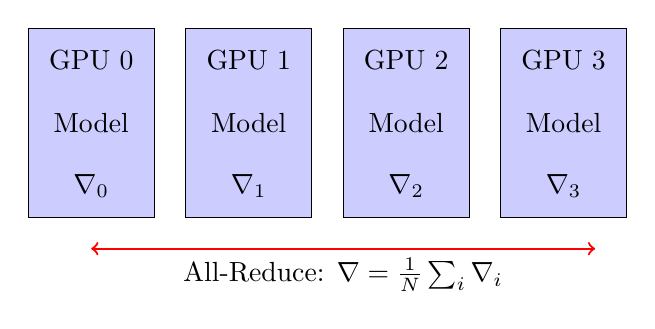
\begin{tikzpicture}[scale=0.8]
    % GPUs
    \foreach \i in {0,1,2,3} {
        \draw[fill=blue!20] (\i*2.5, 0) rectangle (\i*2.5+2, 3);
        \node at (\i*2.5+1, 2.5) {GPU \i};
        \node at (\i*2.5+1, 1.5) {Model};
        \node at (\i*2.5+1, 0.5) {$\nabla_\i$};
    }

    % All-Reduce
    \draw[<->, thick, red] (1, -0.5) -- (9, -0.5);
    \node[below] at (5, -0.5) {All-Reduce: $\nabla = \frac{1}{N}\sum_i \nabla_i$};
\end{tikzpicture}
\caption{数据并行:每个GPU持有完整模型,梯度通过All-Reduce同步}
\label{fig:data_parallel}
\end{figure}

\subsubsection{PyTorch DDP}

PyTorch的\texttt{DistributedDataParallel}(DDP)是标准的数据并行实现:
\begin{itemize}
    \item 使用NCCL后端进行高效GPU通信
    \item 梯度计算与通信重叠(Overlap)
    \item 支持梯度桶(Gradient Bucketing)优化
\end{itemize}

\textbf{局限}:每个GPU必须能容纳完整模型,无法训练超大模型。

\subsection{ZeRO:零冗余优化器}

ZeRO(Zero Redundancy Optimizer)~\citep{rajbhandari2020zero}是DeepSpeed的核心技术,通过分片消除数据并行中的内存冗余。

\subsubsection{三个阶段}

\paragraph{ZeRO-1:优化器状态分片}
将Adam的$m, v$和FP32参数副本分片到$N$个GPU:
\begin{equation}
    \text{优化器显存}: 12\Phi \to \frac{12\Phi}{N}
\end{equation}
每个GPU只更新$1/N$的参数,通过All-Gather获取完整参数。

\textbf{显存节省}:约$4\times$(相比普通DP)

\paragraph{ZeRO-2:+ 梯度分片}
梯度也按$1/N$分片,每个GPU只保留与其优化器分片对应的梯度:
\begin{equation}
    \text{梯度显存}: 2\Phi \to \frac{2\Phi}{N}
\end{equation}
使用Reduce-Scatter替代All-Reduce。

\textbf{显存节省}:约$8\times$

\paragraph{ZeRO-3:+ 参数分片}
模型参数也分片,前向/反向传播时按需All-Gather:
\begin{equation}
    \text{参数显存}: 2\Phi \to \frac{2\Phi}{N}
\end{equation}
\textbf{显存节省}:约$N\times$(线性扩展)

\begin{table}[htbp]
\centering
\caption{ZeRO各阶段显存占用对比($N$个GPU)}
\label{tab:zero_stages}
\begin{tabular}{lccc}
\toprule
阶段 & 分片内容 & 单GPU显存 & 通信量 \\
\midrule
DDP & 无 & $16\Phi$ & $2\Phi$ \\
ZeRO-1 & 优化器状态 & $4\Phi + 12\Phi/N$ & $2\Phi$ \\
ZeRO-2 & + 梯度 & $2\Phi + 14\Phi/N$ & $2\Phi$ \\
ZeRO-3 & + 参数 & $16\Phi/N$ & $3\Phi$ \\
\bottomrule
\end{tabular}
\end{table}

\subsubsection{ZeRO-Offload与ZeRO-Infinity}

\paragraph{ZeRO-Offload}
将优化器状态和计算卸载到CPU:
\begin{itemize}
    \item GPU只保留FP16参数和梯度
    \item CPU负责FP32参数更新
    \item 单GPU可训练10B+模型
\end{itemize}

\paragraph{ZeRO-Infinity}
进一步卸载到NVMe SSD:
\begin{itemize}
    \item 利用NVMe的大容量(TB级)
    \item 512 GPU可训练万亿参数模型
    \item 带宽优化:预取、分层缓存
\end{itemize}

\subsection{模型并行}

当单个模型层无法放入单GPU时,需要模型并行。

\subsubsection{张量并行(Tensor Parallelism)}

张量并行~\citep{shoeybi2019megatron}将单个层的参数矩阵切分到多个GPU。

\paragraph{MLP层的张量并行}

对于FFN层 $Y = \text{GeLU}(XW_1)W_2$:

\textbf{列切分}$W_1$(沿输出维度):
\begin{equation}
    W_1 = [W_1^{(1)}, W_1^{(2)}], \quad Y_1 = \text{GeLU}(X W_1^{(i)})
\end{equation}
每个GPU独立计算部分输出,无需通信。

\textbf{行切分}$W_2$(沿输入维度):
\begin{equation}
    W_2 = \begin{bmatrix} W_2^{(1)} \\ W_2^{(2)} \end{bmatrix}, \quad Y = \sum_i Y_1^{(i)} W_2^{(i)}
\end{equation}
需要All-Reduce求和。

\begin{figure}[htbp]
\centering
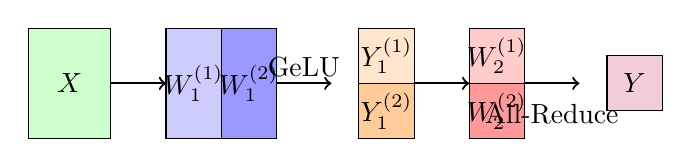
\begin{tikzpicture}[scale=0.7]
    % Input X
    \draw[fill=green!20] (0, 0) rectangle (1.5, 2);
    \node at (0.75, 1) {$X$};

    % W1 column split
    \draw[fill=blue!20] (2.5, 0) rectangle (3.5, 2);
    \draw[fill=blue!40] (3.5, 0) rectangle (4.5, 2);
    \node at (3, 1) {$W_1^{(1)}$};
    \node at (4, 1) {$W_1^{(2)}$};

    % GeLU outputs
    \draw[fill=orange!20] (6, 1) rectangle (7, 2);
    \draw[fill=orange!40] (6, 0) rectangle (7, 1);
    \node at (6.5, 1.5) {$Y_1^{(1)}$};
    \node at (6.5, 0.5) {$Y_1^{(2)}$};

    % W2 row split
    \draw[fill=red!20] (8, 1) rectangle (9, 2);
    \draw[fill=red!40] (8, 0) rectangle (9, 1);
    \node at (8.5, 1.5) {$W_2^{(1)}$};
    \node at (8.5, 0.5) {$W_2^{(2)}$};

    % Output
    \draw[fill=purple!20] (10.5, 0.5) rectangle (11.5, 1.5);
    \node at (11, 1) {$Y$};

    % Arrows
    \draw[->, thick] (1.5, 1) -- (2.5, 1);
    \draw[->, thick] (4.5, 1) -- (5.5, 1);
    \node at (5, 1.3) {GeLU};
    \draw[->, thick] (7, 1) -- (8, 1);
    \draw[->, thick] (9, 1) -- (10, 1);
    \node[below] at (9.5, 0.8) {All-Reduce};
\end{tikzpicture}
\caption{MLP层的张量并行:$W_1$列切分,$W_2$行切分}
\label{fig:tensor_parallel_mlp}
\end{figure}

\paragraph{注意力层的张量并行}

多头注意力天然适合张量并行:
\begin{itemize}
    \item 将$h$个头分配到$N$个GPU,每个GPU处理$h/N$个头
    \item $Q, K, V$投影矩阵按头切分(列切分)
    \item 输出投影$W_O$按行切分
    \item 前向需要1次All-Reduce,反向需要1次All-Reduce
\end{itemize}

\paragraph{通信开销}
每个Transformer层需要:
\begin{itemize}
    \item 前向:2次All-Reduce(注意力 + MLP)
    \item 反向:2次All-Reduce
\end{itemize}

张量并行适合\textbf{节点内}高带宽互连(NVLink: 600GB/s)。

\subsubsection{序列并行(Sequence Parallelism)}

序列并行~\citep{korthikanti2023reducing}在序列维度切分,减少激活显存:

\begin{itemize}
    \item LayerNorm和Dropout在序列维度独立,可以分片
    \item 与张量并行配合:TP区域外使用SP
    \item 将All-Reduce拆分为Reduce-Scatter + All-Gather
\end{itemize}

\textbf{优势}:激活显存降低$N$倍($N$为TP度),无额外通信。

\subsubsection{流水线并行(Pipeline Parallelism)}

流水线并行~\citep{huang2019gpipe}将模型按层切分到不同GPU:

\begin{itemize}
    \item GPU 0:Layer 0-7
    \item GPU 1:Layer 8-15
    \item ...
\end{itemize}

\paragraph{朴素流水线的问题}
顺序执行导致严重的\textbf{流水线气泡}(Pipeline Bubble):
\begin{equation}
    \text{气泡比例} = \frac{p - 1}{m + p - 1}
\end{equation}
其中$p$是流水线阶段数,$m$是micro-batch数。

\paragraph{GPipe调度}
将mini-batch切分为多个micro-batch,增大$m$减少气泡:
\begin{itemize}
    \item $m \gg p$时气泡可忽略
    \item 但需要存储所有micro-batch的激活,显存压力大
\end{itemize}

\paragraph{1F1B调度}
一个前向、一个反向交替执行:
\begin{itemize}
    \item 稳态时每个GPU同时有1个micro-batch在前向、1个在反向
    \item 激活显存只需存储$p$个micro-batch
    \item 气泡比例与GPipe相同,但显存更低
\end{itemize}

\begin{figure}[htbp]
\centering
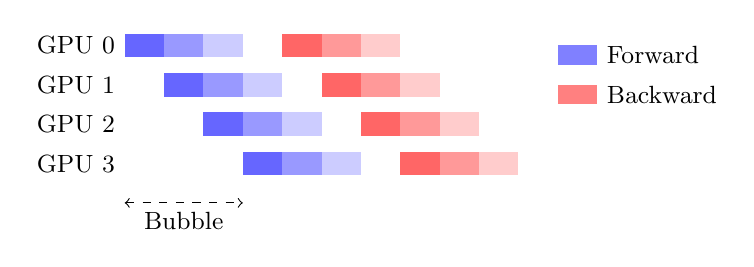
\begin{tikzpicture}[scale=0.5, font=\small]
    % Timeline labels
    \node[left] at (0, 3) {GPU 0};
    \node[left] at (0, 2) {GPU 1};
    \node[left] at (0, 1) {GPU 2};
    \node[left] at (0, 0) {GPU 3};

    % 1F1B schedule (simplified)
    % GPU 0
    \fill[blue!60] (0, 2.7) rectangle (1, 3.3);
    \fill[blue!40] (1, 2.7) rectangle (2, 3.3);
    \fill[blue!20] (2, 2.7) rectangle (3, 3.3);
    \fill[red!60] (4, 2.7) rectangle (5, 3.3);
    \fill[red!40] (5, 2.7) rectangle (6, 3.3);
    \fill[red!20] (6, 2.7) rectangle (7, 3.3);

    % GPU 1
    \fill[blue!60] (1, 1.7) rectangle (2, 2.3);
    \fill[blue!40] (2, 1.7) rectangle (3, 2.3);
    \fill[blue!20] (3, 1.7) rectangle (4, 2.3);
    \fill[red!60] (5, 1.7) rectangle (6, 2.3);
    \fill[red!40] (6, 1.7) rectangle (7, 2.3);
    \fill[red!20] (7, 1.7) rectangle (8, 2.3);

    % GPU 2
    \fill[blue!60] (2, 0.7) rectangle (3, 1.3);
    \fill[blue!40] (3, 0.7) rectangle (4, 1.3);
    \fill[blue!20] (4, 0.7) rectangle (5, 1.3);
    \fill[red!60] (6, 0.7) rectangle (7, 1.3);
    \fill[red!40] (7, 0.7) rectangle (8, 1.3);
    \fill[red!20] (8, 0.7) rectangle (9, 1.3);

    % GPU 3
    \fill[blue!60] (3, -0.3) rectangle (4, 0.3);
    \fill[blue!40] (4, -0.3) rectangle (5, 0.3);
    \fill[blue!20] (5, -0.3) rectangle (6, 0.3);
    \fill[red!60] (7, -0.3) rectangle (8, 0.3);
    \fill[red!40] (8, -0.3) rectangle (9, 0.3);
    \fill[red!20] (9, -0.3) rectangle (10, 0.3);

    % Legend
    \fill[blue!50] (11, 2.5) rectangle (12, 3);
    \node[right] at (12, 2.75) {Forward};
    \fill[red!50] (11, 1.5) rectangle (12, 2);
    \node[right] at (12, 1.75) {Backward};

    % Bubble annotation
    \draw[<->, dashed] (0, -1) -- (3, -1);
    \node[below] at (1.5, -1) {Bubble};
\end{tikzpicture}
\caption{1F1B流水线调度示意图}
\label{fig:1f1b}
\end{figure}

\subsection{3D并行}

Megatron-LM~\citep{narayanan2021efficient}将DP、TP、PP组合成\textbf{3D并行}:

\begin{equation}
    \text{总GPU数} = N_{DP} \times N_{TP} \times N_{PP}
\end{equation}

\subsubsection{并行度选择原则}

\begin{enumerate}
    \item \textbf{TP优先用于节点内}:NVLink带宽高,TP通信频繁
    \item \textbf{PP用于节点间}:通信量小(只传激活),可跨节点
    \item \textbf{DP扩展吞吐}:通信可与计算重叠
\end{enumerate}

\begin{table}[htbp]
\centering
\caption{3D并行配置示例}
\label{tab:3d_parallel}
\begin{tabular}{lccccc}
\toprule
模型 & GPU数 & TP & PP & DP & 配置说明 \\
\midrule
GPT-3 175B & 1024 & 8 & 8 & 16 & 8 GPU/节点 \\
LLaMA-70B & 64 & 8 & 2 & 4 & 单节点8卡 \\
DeepSeek-V3 & 2048 & 8 & - & 256 & MoE+EP \\
\bottomrule
\end{tabular}
\end{table}

\subsection{PyTorch FSDP}

Fully Sharded Data Parallel(FSDP)~\citep{zhao2023pytorch}是PyTorch原生的ZeRO-3实现。

\subsubsection{核心特性}

\begin{itemize}
    \item \textbf{参数分片}:模型参数、梯度、优化器状态全部分片
    \item \textbf{按需All-Gather}:前向/反向时临时恢复完整参数
    \item \textbf{Reduce-Scatter梯度}:反向后立即分片梯度
    \item \textbf{与torch.compile兼容}:可获得额外加速
\end{itemize}

\subsubsection{分片策略}

FSDP支持多种分片粒度:
\begin{itemize}
    \item \texttt{FULL\_SHARD}:完全分片(类似ZeRO-3)
    \item \texttt{SHARD\_GRAD\_OP}:只分片梯度和优化器(类似ZeRO-2)
    \item \texttt{NO\_SHARD}:不分片(类似DDP)
    \item \texttt{HYBRID\_SHARD}:节点内分片,节点间复制
\end{itemize}

\subsubsection{FSDP2}

PyTorch 2.4引入的FSDP2改进:
\begin{itemize}
    \item \textbf{Per-parameter分片}:更细粒度的控制
    \item \textbf{Selective Activation Checkpointing}:选择性重计算
    \item \textbf{SimpleFSDP}:编译器优化版本,吞吐提升可达68\%
\end{itemize}

\subsubsection{FSDP vs DeepSpeed ZeRO}

\begin{table}[htbp]
\centering
\caption{FSDP与DeepSpeed ZeRO对比}
\label{tab:fsdp_vs_zero}
\begin{tabular}{lcc}
\toprule
特性 & PyTorch FSDP & DeepSpeed ZeRO \\
\midrule
原生支持 & PyTorch内置 & 独立库 \\
CPU Offload & 支持 & 支持 \\
NVMe Offload & 有限 & ZeRO-Infinity \\
torch.compile & 兼容 & 有限 \\
配置复杂度 & 较低 & 较高 \\
生态集成 & HuggingFace等 & 广泛 \\
\bottomrule
\end{tabular}
\end{table}

\subsection{混合精度训练}

混合精度训练~\citep{micikevicius2018mixed}使用低精度(FP16/BF16)加速计算,同时保持训练稳定性。

\subsubsection{数值格式对比}

\begin{table}[htbp]
\centering
\caption{浮点数格式对比}
\label{tab:float_formats}
\begin{tabular}{lccccc}
\toprule
格式 & 位数 & 指数位 & 尾数位 & 动态范围 & 精度 \\
\midrule
FP32 & 32 & 8 & 23 & $\pm 3.4 \times 10^{38}$ & 高 \\
FP16 & 16 & 5 & 10 & $\pm 6.5 \times 10^{4}$ & 中 \\
BF16 & 16 & 8 & 7 & $\pm 3.4 \times 10^{38}$ & 低 \\
FP8 (E4M3) & 8 & 4 & 3 & $\pm 448$ & 很低 \\
FP8 (E5M2) & 8 & 5 & 2 & $\pm 5.7 \times 10^{4}$ & 极低 \\
\bottomrule
\end{tabular}
\end{table}

\subsubsection{Loss Scaling}

FP16的动态范围小,梯度可能下溢。\textbf{Loss Scaling}将损失放大:
\begin{align}
    \tilde{L} &= s \cdot L \quad \text{(放大损失)} \\
    \tilde{g} &= \nabla \tilde{L} = s \cdot \nabla L \quad \text{(放大梯度)} \\
    g &= \tilde{g} / s \quad \text{(更新前还原)}
\end{align}

\textbf{动态Loss Scaling}:
\begin{itemize}
    \item 若无溢出,增大$s$(如$s \gets 2s$)
    \item 若发生溢出(NaN/Inf),减小$s$并跳过此步更新
\end{itemize}

\subsubsection{BF16的优势}

BF16与FP32有相同的指数位,因此:
\begin{itemize}
    \item \textbf{无需Loss Scaling}:动态范围与FP32相同
    \item \textbf{训练更稳定}:不会因范围问题溢出
    \item \textbf{精度略低}:尾数只有7位(FP16有10位)
\end{itemize}

现代框架(PyTorch AMP、DeepSpeed)在支持的硬件上默认使用BF16。

\subsubsection{FP8训练}

FP8需要\textbf{每张量缩放}(Per-tensor Scaling):
\begin{itemize}
    \item 每个FP8张量有独立的缩放因子
    \item NVIDIA Transformer Engine自动管理缩放
    \item 需要torch.compile才能获得加速
    \item H100上可比BF16快约10\%
\end{itemize}

\subsection{激活检查点}

激活检查点(Activation Checkpointing)~\citep{chen2016training}通过重计算节省激活显存。

\subsubsection{原理}

前向传播时不保存中间激活,反向传播时重新计算:
\begin{itemize}
    \item \textbf{无检查点}:保存所有激活,显存$O(N)$
    \item \textbf{全检查点}:只保存输入,显存$O(1)$,计算$2\times$
    \item \textbf{$\sqrt{N}$检查点}:每$\sqrt{N}$层设检查点,显存$O(\sqrt{N})$
\end{itemize}

\subsubsection{选择性检查点}

并非所有操作都值得重计算:
\begin{itemize}
    \item \textbf{重计算}:便宜的操作(LayerNorm、激活函数、Dropout)
    \item \textbf{保存}:昂贵的操作(矩阵乘法、注意力)
\end{itemize}

PyTorch的Selective Activation Checkpointing(SAC)支持细粒度控制。

\subsubsection{注意力重计算}

注意力层的激活显存是$O(N^2)$($N$为序列长度),占比最大。FlashAttention通过:
\begin{itemize}
    \item 前向时只保存$(m, \ell)$统计量
    \item 反向时重计算注意力矩阵
\end{itemize}
实现了激活显存$O(N)$,是目前最高效的注意力重计算方案。

\subsection{集合通信}

分布式训练依赖高效的集合通信原语。

\subsubsection{常用通信原语}

\begin{table}[htbp]
\centering
\caption{集合通信原语}
\label{tab:collective_ops}
\begin{tabular}{lll}
\toprule
原语 & 功能 & 应用场景 \\
\midrule
Broadcast & 一对多广播 & 参数初始化 \\
Reduce & 多对一归约 & 梯度聚合到一个节点 \\
All-Reduce & 归约后广播 & DDP梯度同步 \\
All-Gather & 收集所有分片 & ZeRO参数恢复 \\
Reduce-Scatter & 归约后分片 & ZeRO梯度分片 \\
All-to-All & 全交换 & MoE专家通信 \\
\bottomrule
\end{tabular}
\end{table}

\subsubsection{Ring All-Reduce}

Ring All-Reduce是带宽最优的All-Reduce算法:
\begin{enumerate}
    \item \textbf{Reduce-Scatter阶段}:每个GPU向下一个发送$1/N$数据,接收并累加
    \item \textbf{All-Gather阶段}:每个GPU广播自己的归约结果
\end{enumerate}

\textbf{通信量}:$2(N-1)/N \cdot D \approx 2D$($D$为数据量),与GPU数$N$无关。

\textbf{延迟}:$O(N)$步,随GPU数线性增长(延迟非最优)。

\subsubsection{NCCL}

NVIDIA Collective Communication Library(NCCL)是GPU集群通信的标准库:
\begin{itemize}
    \item 自动选择最优拓扑(Ring、Tree、NVLink等)
    \item 支持多节点、多GPU
    \item 与CUDA深度集成
\end{itemize}

\subsection{训练框架对比}

\begin{table}[htbp]
\centering
\caption{主流训练框架对比}
\label{tab:training_frameworks}
\begin{tabular}{lccccc}
\toprule
框架 & 维护方 & TP & PP & ZeRO/FSDP & 特点 \\
\midrule
Megatron-LM & NVIDIA & \checkmark & \checkmark & ZeRO & 3D并行先驱 \\
DeepSpeed & Microsoft & \checkmark & \checkmark & ZeRO-3 & Offload、Infinity \\
PyTorch FSDP & Meta & - & - & FSDP & 原生集成 \\
Alpa & UC Berkeley & \checkmark & \checkmark & - & 自动并行 \\
ColossalAI & HPC-AI & \checkmark & \checkmark & ZeRO & 易用性 \\
\bottomrule
\end{tabular}
\end{table}

\subsection{实践建议}

\paragraph{小模型(< 10B)}
\begin{itemize}
    \item 单卡能放下:使用DDP
    \item 单卡放不下:使用FSDP或ZeRO-2
\end{itemize}

\paragraph{中等模型(10B - 100B)}
\begin{itemize}
    \item 单节点:FSDP/ZeRO-3 + 激活检查点
    \item 多节点:3D并行(TP=8节点内,PP跨节点)
\end{itemize}

\paragraph{超大模型(100B+)}
\begin{itemize}
    \item 必须使用3D并行
    \item 结合专家并行(MoE)
    \item 考虑FP8混合精度
\end{itemize}

\begin{remark}[通信与计算的权衡]
增加并行度会增加通信开销:
\begin{itemize}
    \item TP通信最频繁,应限制在高带宽节点内
    \item PP有气泡开销,需要足够的micro-batch
    \item ZeRO-3的通信量是DDP的1.5倍
\end{itemize}
最优配置需要根据具体硬件和模型进行调优。
\end{remark}

